\documentclass[a4paper]{article}

\usepackage[portuguese]{babel}
\usepackage{comment}
\usepackage[T1]{fontenc}
\usepackage[utf8]{inputenc}
\usepackage{hyperref}
\usepackage{graphicx}
\usepackage{float}
\usepackage{multirow}
\usepackage[hypcap]{caption} % makes \ref point to top of figures and tables
\usepackage{amsmath}
%\usepackage{pdflscape}	% landscape pages
%\usepackage{subcaption}

\title{Projecto 3 --- Adenda}
\author{Gonçalo Ribeiro, 73294\hspace{8mm}Rafael Gonçalves, 73786}

\begin{document}
\maketitle
%\begin{titlepage}

\begin{center}


\includegraphics[width=6cm]{./title}\\[3cm]

\textsc{\LARGE Projecto de Sistemas Digitais}\\[1.5cm]

\textsc{\Large Laboratório 2}\\[1.5cm]


{ \huge \bfseries Escalonamento e Partilha de Recursos \\[3cm] }


\noindent
\begin{minipage}{0.4\textwidth}
\begin{flushleft} \large
Rafael Gonçalves, 73786
\end{flushleft}
\end{minipage}
\begin{minipage}{0.4\textwidth}
\begin{flushright} \large
Gonçalo Ribeiro, 73294
\end{flushright}
\end{minipage}

\vfill

{\large \today}


\end{center}

\end{titlepage}

%\tableofcontents

\section{Resumo}
O presente documento é uma adenda ao relatório entregue no dia 21 de Dezembro de 2014.

À data de entrega do relatório a unidade HALF estava concluída; e do SAVE faltava afinar a máquina de estados. Faltava também ligar as BRAMs, e fazer a máquina de estados que pede input ao utilizador.

Os pontos que se seguem resumem as alterações que foram feitas em relação à data de entrega do relatório.

\begin{itemize}
	\item redesenhou-se a unidade de armazenamento;
	\item adicionou-se uma segunda FSM ao módulo SAVE, que permite tratar correctamente as operações compostas;
	\item desenhou-se a FSM que permite ao utilizador introduzir os parâmetros largura, altura e tipo de operação;
	\item fizeram-se as ligações às BRAMs.
\end{itemize}

\section{Detalhes das Alterações}

\subsection*{Unidade de Armazenamento}

A unidade de armazenamento anteriormente projectada usava muitos multiplexers, o que se traduzia numa grande ocupação de hardware. Eram utilizados cerca de 224 multiplexers 4:1.

O desenho era extremamente ineficiente. Em vez de alterar o fluxo de dados dentro da Unidade de Armazenamento, o novo desenho selecciona de dentro da UA quais os conjuntos de dados a fazer sair, diminuindo o hardware mas obtendo exactamente a mesma funcionalidade que o anterior.

No novo desenho existem apenas 64 multiplexers 4:1.


\subsection*{FSM do SAVE}

A Máquina de Estados do SAVE foi completamente redesenhada, dividindo-se agora em duas (uma que funciona sempre e uma segunda que só funciona nas operações compostas).

A primeira máquina de estados gere a Unidade de Armazenamento Principal e a primeira unidade funcional em uso, e a segunda gere a UA Secundária, bem como a segunda unidade funcional.

Uma vez feitos os atrasos condicionais (via multiplexer) dos sinais relevantes, sincronizou-se o SAVE com o HALF.

\subsection*{FSM de Input}

A FSM de input permite ao utilizador inserir a largura e altura da imagem bem como a operação morfológica que pretende. Decidiu-se usar o botão 0 para \textit{reset} e o botão 1 para confirmar a inserção de cada parâmetro e mandar iniciar a transformação.

A máquina de estados resultante é a da \autoref{fig:FSMinput}. No estado \texttt{start} o processamento da imagem começa. Quando a imagem acaba de ser processada a FSM passa ao estado \texttt{end}.

\begin{figure}
	\centering
	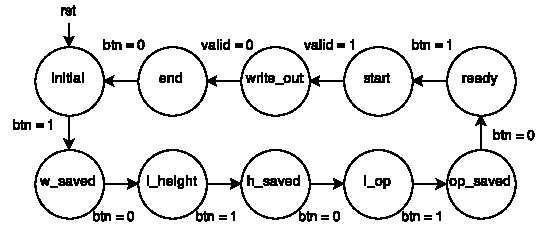
\includegraphics[width=.9\textwidth]{controlo_FSM}
	\caption{FSM de input. Por omissão o estado não muda.}
	\label{fig:FSMinput}
\end{figure}

\subsection*{Ligação às BRAMs}
Para usar as BRAMs, os ficheiros \texttt{BlockRam.vhd} e \texttt{usb2bram.vhd} foram alterados. No primeiro passou a usar-se a RAMB16\_S9\_S36, ou seja uma BRAM com 512 posições de memória cada uma com 32 bits (mais bits de paridade). Como a largura das palavras foi alterada, no ficheiro \texttt{usb2bram.vhd} alterou-se a largura das \textit{buses} de dados dos portos B para 32 bits e a largura dos endereços desses portos para 9 bits.

De seguida, o ficheiro \texttt{controlo.vhd} foi substituido por outro contendo a FSM correspondente à \autoref{fig:FSMinput}; e \texttt{datapath.vdh} foi substituido por um componente que agrega as FSMDs do HALF e SAVE.

\section{Falhas}

Uma vez integradas as FSMDs no circuito com as BRAMs, detectou-se em simulação (e posteriormente em implementação) que não havia sincronismo na leitura da memória. Apesar dessa falha, era possível verificar que as 5 operações eram realizadas correctamente sobre os valores de inicialização das memórias.

\end{document}
